\documentclass[%
a4paper,%
11pt,%
DIV12,%
BCOR20mm,%
twoside,%
openright,%
headsepline,%
bibtotocnumbered%
]{scrbook}

%%% Sprach-Konfiguration
\usepackage[utf8]{inputenc}
\usepackage[ngerman]{babel}
\hyphenation{whe-ther}
\usepackage{microtype}% verbesserter Randausgleich

%%% Grafik-Konfiguration
\usepackage{graphicx}
%\usepackage[hang]{subfigure}     % Subfigures if you need them
\usepackage{rotating}             % you can place sidewaysfigures with this!
\usepackage[format=hang]{caption} % Better-looking captions

%%% Schriftarten und Symbole
\usepackage[T1]{fontenc}

% -- Use this if you want some nicer fonts --
\usepackage{mathptmx}
\usepackage[scaled=0.9]{helvet}
% \usepackage{courier}            % I don't like courier, ascii looks better
\usepackage{ascii}

%%% Mathematik
\usepackage{amsmath}
\usepackage{amssymb}

%%% Sonstiges
\usepackage[below]{placeins}                   % Manages Floats
%\usepackage{calc}
\usepackage{ifthen}                            % Needed for macros
%\usepackage{url}                              % Typeset clickable URL's 
\usepackage{xspace}                            % Useful for macros!
\usepackage[printonlyused]{acronym}   % Acronym management package
\usepackage{blindtext}                         % Generates 'Lorem Ipsum' for this template
\usepackage{booktabs}                          % Typesets optimal tables; see documentation

\usepackage{tikz}                              % If you want to use TikZ for some figures
\input{img/tikzsetup}                          % See img/tikzsetup.tex for further explanations

%%% If you need code-listings
%\usepackage{listings}
%\lstloadlanguages{C}
%\lstset{%
%language=C,%
%basicstyle=\ttfamily\small,%
%keywordstyle=\bfseries,%
%identifierstyle=,%
%commentstyle=\itshape,%
%showstringspaces=false,%
%numbers=left,%
%numberstyle=\ttfamily\footnotesize,%
%numbersep=1em,%
%xleftmargin=12mm,%
%breaklines=true,%
%breakatwhitespace=true,%
%}

%%% Set up PDF-Stuff
%%% Set up hyperref if we are compiling with pdflatex
%%
\ifx\pdftexversion\undefined
\usepackage{hyperref}
\else
\usepackage[colorlinks=false,       %true => text des links wird farbig, false => farbiges kaestchen (wird nicht gedruckt) um schwarzen text
            linkcolor=black,        %nur bei colorlinks=true
            urlcolor=black,
            citecolor=black,
            bookmarks,                  % Bookmarks erstellen
            bookmarksopen=true,         % Bookmark beim Oeffnen anzeigen?
            pdfpagemode=UseOutlines,    % Bookmark beim Oeffnenanzeigen? (UseOutlines / none)
            bookmarksopenlevel=3,       % bis zu welcher Ebenen geoeffnet
            bookmarksnumbered,          % Kapitelnummern in Bookmarks
            pdftitle={Erkennung körperlicher Aktivitäten mittels Smartphone- und Smartwatch-Sensoren und Machine Learning},
            pdfsubject={Bachelorarbeit},
            pdfkeywords={Smartphone, Smartwatch, Bachelorarbeit, Machine Learning, Aktivitätenerkennung},
            pdfauthor={Christian Brüggemann}
            ]{hyperref}
\fi

%%% 
%%
\ifx\pdftexversion\undefined
\else
\pdfminorversion=6
\pdfoutput=1        % PDF-Ausgabe anschalten.
\pdfimageresolution=600
\pdfcompresslevel=5 % 0 keine kompression, 9 staerkste kompression
\fi

% vim: set ft=tex
  % Customize pdfsetup.tex

%%% Set up the Title
%%% Daten für die Titelseite. Bitte korrekt ausfüllen. ;-)
%%
\newcommand{\Title}{Erkennung körperlicher Aktivitäten mittels Smartphone- und Smartwatch-Sensoren und Machine Learning}
\newcommand{\Type}{Bachelorarbeit}
\newcommand{\Author}{\href{mailto:cbruegg@mail.upb.de}{Christian Brüggemann}}
\newcommand{\Strasse}{Salbeiweg 39}
\newcommand{\Matrikelnummer}{7004878}
\newcommand{\Ort}{33100 Paderborn}
\newcommand{\BetreuerA}{\href{mailto:artus@aisbi.de}{Jun.-Prof. Dr. Artus Krohn-Grimberghe}}
\newcommand{\Zweitgutachter}{\href{mailto:eyke@upb.de}{Prof.\ Dr.\ Eyke Hüllermeier}}
\newcommand{\Date}{22.03.2017}


%%% ------- DO NOT MODIFY BELOW HERE --------
%%
\newcommand{\Maketitle}{%
%
\titlehead{%
\includegraphics[scale=0.4]{img/uni-logo-woname}%
\hfill%
\raisebox{1em}{
\parbox[c]{10cm}{%
\begin{center}
  Universität Paderborn --- Fakultät Wirtschaftswissenschaften \\
  Fachgebiet Analytic Information Systems and Business Intelligence \\
  Jun.-Prof.\ Dr.\ Artus Krohn-Grimberghe
\end{center}%
}}\hfill%
\includegraphics*[width=0.1\textwidth]{img/logo_aisbi}
}
%
\subject{%
\Type
}
%
\title{\Title}
\author{\Author}
\date{\Date}
\publishers{Betreut von: \\ \BetreuerA}

\uppertitleback{%
\textbf{\Type} \\
extern am Fachgebiet Analytic Information Systems and Business Intelligence \\
Fakultät Wirtschaftswissenschaften \\
Jun-.Prof. Dr. Artus Krohn-Grimberghe \\[1em]
Institut für Informatik\\
Fakultät für Elektrotechnik, Informatik und Mathematik\\
Universität Paderborn \\[2em]
Vorgelegt von: \\
\Author \\
Matrikelnummer: \Matrikelnummer \\
\Strasse \\
\Ort\\[1em]
am \\
\Date \\[2em]
Betreut durch:\\
\BetreuerA \\
Zweitgutachter:\\
\Zweitgutachter
}
\maketitle%
}
% vim: set ft=tex
 % Customize titlesetup.tex for a nice title

%%% Input own Macro's
% Create your own macros here!

%% Place a figure
% 1.) alt-caption (for lof)
% 2.) caption
% 3.) label
% 4.) figure placement (htbp)
% 5.) figure content
\newcommand{\FIG}[5][]{
  \begin{figure}[#4]
  \centering
  #5 
  \ifthenelse{\equal{#1}{}}{%
    \caption{#2}
  }{%
    \caption[#1]{#2}
  }
  \label{fig:#3}
  \end{figure}%
}

%% Place a sideways figure
% 1.) alt-caption (for lof)
% 2.) caption
% 3.) label
% 4.) figure placement (htbp)
% 5.) figure content
\newcommand{\SFIG}[5][]{
  \begin{sidewaysfigure}[#4]
  \centering
  #5 
  \ifthenelse{\equal{#1}{}}{%
    \caption{#2}
  }{%
    \caption[#1]{#2}
  }
  \label{fig:#3}
  \end{sidewaysfigure}%
}

% vim: set ft=tex

% todocommand
\newcommand{\todo}[1]{}
\renewcommand{\todo}[1]{{\color{red} TODO: {#1}}}


%%% Which Chapters to include in draft. Commentate for production.
%\includeonly{%
%abstract,%
%introduction,%
%background,%
%design,%
%implementation,%
%performancestudy,%
%conclusions,%
%appendixA,%
%appendixB%
%}

%%%
\begin{document}
%\input{lsthack}  % Uncomment if you use listings !!!
\frontmatter
\Maketitle
\todo{FG-Logo ändern}

\chapter*{Zusammenfassung}
Handelsübliche Smartphones und Smartwatches, sowie Fitness-Tracker enthalten Sensoren, mit denen sich die körperlichen Aktivitäten des Benutzers aufzeichnen und auswerten lassen. Frühere Forschung widmete sich bereits der Aktivitätenerkennung mittels Smartphones und Smartwatches, jedoch wurden die Daten bisher voneinander getrennt behandelt. Diese Bachelorarbeit widmet sich der Kombination der Datenquellen, um die Vorteile beider Gerätetypen zu vereinen und Modelle mittels maschinellem Lernen zu bilden, die sowohl handorientierte als auch allgemeine Aktivitäten mit hoher Genauigkeit klassifizieren können. Die entwickelte Methode wurde anhand eines Datensatzes ausgewertet, der im Rahmen dieser Arbeit durch ein Experiment mit 10 Personen aufgenommen wurde.

% vim: set ft=tex

\acresetall       % Reset all acronyms

\tableofcontents
\listoffigures
%\listoftables      % Uncomment if you have tables
%\lstlistoflistings % Uncomment if you use listings

\mainmatter

\chapter{Einleitung}
\label{chap:introduction}
\section{Motivation}
Smartphones haben im letzten Jahrzehnt an großer Bedeutung gewonnen. Daneben existieren mittlerweile ergänzend dazu sogenannte \textit{Smartwatches} und \textit{Fitness-Tracker}. Smartwatches sind Armbanduhren, die in der Regel drahtlos mit einem Smartphone verbunden sind und Informationen wie beispielsweise Benachrichtigungen am Handgelenk zugänglich machen. Fitness-Tracker besitzen ähnliche Funktionen, zielen allerdings primär darauf ab, die Fitness und Gesundheit des Nutzers zu fördern, indem Daten wie beispielsweise die Schrittanzahl des Nutzers pro Tag gesammelt und grafisch aufbereitet werden. In beiden Geräteformen werden üblicherweise Sensoren verbaut, mit denen sich die Bewegungen des Trägers nachvollziehen lassen.

Mit einigen Fitness-Trackern des Unternehmens \textit{Fitbit} existieren bereits kommerzielle Produkte, die über die reine Sammlung und grafische Aufbereitung von Daten hinausgehen: Die Funktion \textit{SmartTrack} erkennt kontinuierliche Aktivitäten mit hoher Bewegung mit Hilfe von Sensordaten des Trackers teilweise automatisch, ohne dass der Anwender vorher manuell einstellen muss, welcher Aktivität er in den nächsten Minuten nachgehen wird \cite{FitbitSmartTrack}. Dies hat den Vorteil, dass der Nutzer sich nicht daran erinnern muss, im Fitness-Tracker die richtige Aktivität einzustellen, um kategorisierte Statistiken zu erhalten.

SmartTrack unterstützt die folgenden Aktivitäten: Gehen, Laufen, Fahrradfahren, Schwimmen und Training mit einem Crosstrainer, sowie zwei allgemeine Kategorien "Sport" (Fußball, Basketball, Tennis, etc.) und "aerobes Training" (Zumba, Tanzen).

Es existieren weitere mögliche Anwendungsgebiete der automatisierten Aktivitätenerkennung. Für Smartphone-Betriebssysteme könnte das Wissen, dass der Anwender gerade Sport treibt, interessant sein, um eingehende Anrufe eines nicht als wichtig markierten Kontaktes zu unterdrücken. Des Weiteren könnte das Forschungsgebiet der "Transportation Mode Recognition" von solchen Methoden profitieren: Soll erkannt werden, mit welchem Verkehrsmittel sich der Nutzer gerade fortbewegt, könnte neben dem Parameter der Geschwindigkeit ebenfalls von Interesse ein, ob mit Hilfe der Methode die Aktivität "Fahrradfahren" erkannt wird oder nicht. So ließe sich die Fortbewegung mittels eines Mofas von der Fortbewegung mittels eines Fahrrads unterscheiden, was insbesondere für Dienste wie "Google Now" nützlich sein könnte. Diese dienen dem Nutzer als persönlicher Assistent und warnen ihn beispielsweise vor Stau auf einer häufig befahrenen Strecke. Eine solche Warnung könnte entfallen, wenn festgestellt wurde, dass der Nutzer die Strecke nicht mit einem Motorroller, sondern mit einem Fahrrad bewältigt und somit Radwege befahren darf.

In der Literatur ist \cite{Weiss2016} hervorzuheben. Die Autoren vergleichen in ihrem Paper die Genauigkeit der Aktivitätenerkennung eines Smartphones mit der einer Smartwatch und kommen zu dem Schluss, dass die Güte der jeweiligen Erkennung insbesondere von der Aktivität selbst abhängig ist. Es liegt auf der Hand, dass nur mit Hilfe eines Smartphones beispielsweise eine Unterscheidung zwischen "Zähneputzen" und "Stehen" schwer möglich ist, während analog dazu nur mit Hilfe einer Smartwatch die Unterscheidung zwischen "Gehen" und "Fußball schießen" ebenfalls herausfordernd ist. Naheliegend ist daher, eine Kombination beider Datenquellen einzusetzen, um die durchschnittliche Erkennungsrate zu verbessern, ohne eine Beschränkung der erkennbaren Aktivitäten einzuführen.

\section{Ziele der Arbeit} % Problemdefinition
\label{sec:goals}
Evaluiert werden soll ein zu entwickelndes Verfahren, das mit Methoden des \textit{maschinellen Lernens} (siehe Definition~\ref{def:ml-classification}) und eben jenen gesammelten Daten feststellt, welcher Aktivität der Träger der Geräte in bestimmten Zeitintervallen nachgegangen ist. Hierzu wird zunächst eine Software benötigt, welche die synchrone Aufzeichnung von Sensordaten eines Smartphones und zusätzlich eines Fitness-Trackers oder einer Smartwatch ermöglicht.

Es ergibt sich insbesondere die Frage, inwiefern sowohl personalisierte, das heißt nutzerspezifische, als auch unpersonalisierte Modelle durch die Hinzunahme einer weiteren Datenquelle genauer werden.

Um eine Evaluation zu ermöglichen, wird ein Beispieldatensatz benötigt, der durch ein Experiment mit 10 Probanden aufgebaut wird. Orientiert ist diese Zahl an der Anzahl der Probanden in \cite{Weiss2016}, an dessen Experiment 17 Personen teilgenommen haben. Im Experiment sollen diese voneinander unabhängig mehreren definierten Aktivitäten nachgehen, während parallel dazu Sensordaten mithilfe der entwickelten Software aufgezeichnet werden. Um die Vergleichbarkeit mit den Ergebnissen aus \cite{Weiss2016} zu gewährleisten, werden die Probanden in diesem Experiment denselben Aktivitäten nachgehen.

Als Fitness-Tracker wurde das \textit{Microsoft Band 2} ausgewählt, da dieser vom Lehrstuhl für diese Arbeit zur Verfügung gestellt wurde, im Vergleich zur privat vorhandenen Smartwatch \textit{Pebble Time} mehr Sensoren besitzt und letztere während der Durchführung des Experiments nach einem erzwungenen Software-Update falsche Zeitstempel für Sensordaten lieferte. 

\section{Wichtige Ergebnisse}
Hervorzuheben sind die Erkenntnisse, dass die Genauigkeit persönlicher Modelle mithilfe der Kombination der in Abschnitt~\ref{sec:sensors} vorgestellten Sensoren auf $99.4 \%$ gesteigert werden konnte. Im Vergleich zu Modellen, die nur auf Daten des Beschleunigungssensors eines Fitness-Trackers basieren, beträgt die Steigerung damit $7.8$ Prozentpunkte. Unpersönliche Modelle hingegen konnten durch diese Technik um $3.3$ Prozentpunkte auf $78.5 \%$ verbessert werden, wobei gleichzeitig die Stabilität insofern gesteigert wurde, dass die schlechteste Genauigkeit für einen Teilnehmer des Experiments mit einem unpersönlichen Modell nicht unter $64 \%$ lag. Um die Genauigkeit unpersönlicher Modelle weiter zu verbessern, empfiehlt es sich, nur klar voneinander abgrenzbare Aktivitäten zu klassifizieren und beispielsweise mehrere Essaktivitäten zu vermeiden.

Des Weiteren konnte festgestellt werden, dass auch niedrige, einstellige Sensorabtastraten in Hz bei einem niedrigeren Energieverbrauch noch gute Ergebnisse liefern können und die Variation hinsichtlich der Ausrichtung der Geräte nur einen geringen Einfluss auf die Genauigkeiten der Modelle hat.

\section{Struktur dieser Arbeit}
Kapitel~\ref{chap:background} erläutert die verwendeten Sensoren sowie wichtige Begriffe des maschinellen Lernens als Grundlagen dieser Arbeit. Im darauffolgenden Kapitel~\ref{chap:relatedwork} werden verwandte Arbeiten aufgezählt und historisch eingeordnet, da insbesondere die Entwicklung mobiler Technologie diverse Fortschritte im Bereich der Aktivitätenerkennung erst ermöglicht hat. Anschließend daran wird in Kapitel~\ref{chap:experiment} der Aufbau des Experiments beschrieben, das im Rahmen dieser Bachelorarbeit durchgeführt wurde, um die benötigten Daten zu sammeln. Die Verarbeitung der gewonnenen Daten wird in Kapitel~\ref{chap:method} erläutert. Die aus der Anwendung der Methode resultierenden Modelle werden in Kapitel~\ref{chap:evaluation} evaluiert, wobei unter anderem diverse Eigenschaften des aufgenommenen Datensatzes variiert werden, um Erkenntnisse über den Wert der Sensoren für die Aktivitätenerkennung zu erhalten. Ein abschließendes Fazit der Arbeit erfolgt in Kapitel~\ref{chap:conclusions}.

% vim: set ft=tex

\chapter{Grundlagen}
\label{chap:background}
\section{Erläuterung der verwendeten Sensoren}
\todo{Grafiken zur Erläuterung}
Während in der Einleitung nur generisch von "Sensordaten" die Rede war, werden diese nun konkretisiert. Zur Aufnahme werden das Smartphone OnePlus 3 sowie der Fitness-Tracker Microsoft Band 2 verwendet. Beide Geräte besitzen einen Beschleunigungssensor sowie ein Gyroskop. Des Weiteren besitzt das Band unter anderem einen Sensor, der den elektrischen Widerstand der Haut des Trägers misst, sowie einen Hauttemperatursensor.

\subsection{Beschleunigungssensor}
Ein Beschleunigungssensor, auch \textit{Accelerometer} genannt, misst die echte Beschleunigung eines Objektes im Raum je physikalischer Achse ($x$, $y$ und $z$). Dies beinhaltet auch die Beschleunigung, die von der Erdgravitation ausgeht: Liegt das Objekt beispielsweise auf dem Boden, erfährt es auf der im rechten Winkel zum Boden stehenden Achse eine Beschleunigung von $g \approx 9.81$ $m/s^2$\cite{SensorsOverview}\cite{nistsi}. Über diesen Sensor kann demnach die Orientierung des Objektes im Raum bestimmt werden. \\
Die Daten dieses Sensors werden von beiden Geräten aufgezeichnet.

\subsection{Gyroskop}
Ein Gyroskop misst die Rotationsgeschwindigkeit je physikalischer Achse\cite{SensorsOverview}. Demnach bedeutet der Messwert $(x=0, y=0, z=0)$, dass das Objekt relativ zur Erde nicht bewegt wird, während $(x=1, y=0, z=0)$ bedeutet, dass das Objekt um die $x$-Achse gedreht wird. \\
Die Daten dieses Sensors werden von beiden Geräten aufgezeichnet.

\subsection{Hautwiderstandssensor}
Je nach aktueller körperlicher Betätigung ändert sich die elektrische Leitfähigkeit der Hautoberfläche durch Schweiß. Der Hautwiderstandssensor misst den elektrischen Widerstand der Haut, der sich umgekehrt proportional zur Leitfähigkeit verhält.
Dieser Sensor ist nur im Band integriert, das daher für diesen die einzige Datenquelle ist.

\subsection{Hauttemperatursensor}
Der Hauttemperatursensor misst die Temperatur der Haut des Nutzers, die an der Unterseite des Band anliegt. Leider reagierte dieser Sensor in einem Test sogar bereits langsam auf Temperaturveränderungen, wenn das Band abgelegt wurde, sodass auf die Aufzeichnung dieser Daten verzichtet wurde.

\section{Grundlagen der Machine Learning-Klassifikation}
In den folgenden Abschnitten wird von einem grundlegenden Verständnis von Machine Learning-Klassifikation ausgegangen, weshalb wir diese Technik nun kurz erläutern. \\
\todo{put this in an actual definition}
Gegeben sei ein Datensatz $D \ni (x_1, ..., x_n, y)$ mit $|D| = m$ Instanzen. Dann sind $x = (x_1, ..., x_n)$ die \textit{Input Features} und $y$ ist das \textit{Target}. Im Falle eines Klassifikationsproblems ist $y$ nominal, d.h. ein deskriptiver Wert zur Identifikation. Gesucht ist nun eine \textit{Hypothesenfunktion} $h(x) = \hat{y}$, die zu gegebenen Features den wahrscheinlichsten Wert des Targets bestimmt\cite{Ng2011a}.

Ein einfaches Beispiel kann wie folgt konstruiert werden: Sei $x = (x_1)$, wobei $x_1$ die Wohnfläche einer Wohnung oder eines Hauses in $m^2$ ist. Des Weiteren sei $D = \{(50, \text{Wohnung}), (75, \text{Wohnung}), (200, \text{Haus}), (300, \text{Haus})\}$. Eine sinnvolle Hypothesenfunktion wäre in diesem Fall beispielsweise gegeben durch:

\[
h(x) = 
\begin{cases}
\text{Wohnung}, & \text{wenn } x_1 < 200 \\
\text{Haus}, & \text{sonst}
\end{cases}
\]

Das beschriebene Klassifikationsproblem kann mittels Algorithmen des \textit{Machine Learnings} (im Folgenden \textit{ML}) gelöst werden, indem eine Verlustfunktion definiert wird, die ein solcher Algorithmus zu minimieren versucht. Eine solche Verlustfunktion bestraft die fehlerhafte Klassifikation einer Instanz, indem sie einen höheren Wert annimmt.

% vim: set ft=tex

\chapter{Verwandte Arbeiten}
\label{chap:relatedwork}
Dieses Kapitel behandelt verwandte Arbeiten, die bis in das Jahr 1998 zurückreichen. Im November 1998 veröffentlichten Schmidt et al. im Rahmen des \textit{Technology for Enabling Awareness (TEA)}-Projektes ein Paper über \textit{Context Awareness in Ultra-Mobile Computing}, in dem sie darauf hinwiesen, dass Kontext mehr beinhaltet als den Ort des Geschehens, auf den sich vorige Werke konzentrierten \cite{Schmidt1999}. In diesem Paper schlugen sie neben der Verwendung expliziter Regeln zur Erkennung diverser Aktivitäten zusätzlich auch die Verwendung von Methoden künstlicher Intelligenz vor.

Parallel dazu erkannte Ashbrook 1999 ebenfalls die Bedeutung der Kontexterkennung als wichtige Komponente tragbarer Computeranwendungen \cite{Ashbrook1999}. Ein damals kommerziell verfügbares Produkt namens \textit{Twiddler}, eine mit nur einer Hand bedienbare Tastatur, integrierte zwei Sensoren, welche die Ausrichtung des Gerätes feststellen konnten. Mit der Motivation, automatisch eine To-Do-Liste zu öffnen, wenn der Nutzer des Gerätes sich zu seinem nächsten Termin bewegt, untersuchte Ashbrook die Möglichkeit, eben diese Tätigkeit mit Hilfe der genannten Sensoren automatisch erkennen zu lassen. Er schlug mehrere solche Methoden vor, die allerdings allesamt keinen Gebrauch von Machine Learning machten und nur schwer auf andere Aktivitäten übertragbar waren.

Ebenfalls im Jahr 1999 äußerten Farringdon et al. Kritik an Mobilgeräten wie Handys und PDAs, die ihre Besitzer auch in unangemessenen Situationen visuell und akustisch über eingehende Nachrichten benachrichtigen \cite{Farringdon1999}. Um dieses Problem anzugehen entwickelten sie ein an der Hüfte tragbares Gerät, das zwei einachsige Accelerometer integrierte, sowie eine Jacke, die die Dehnung des Materials messen konnte. Auch hier wurde Machine Learning nicht eingesetzt. Stattdessen wurde für die Erkennung der Aktivitäten Sitzen, Stehen, Liegen, Gehen und Laufen ein Algorithmus entwickelt, der Aspekte wie die Durchschnittswerte der Sensoren betrachtet und mit Schwellwerten vergleicht.

\begin{figure}
\centering
\includegraphics[clip,trim=25mm 90mm 110mm 115mm, page=6, scale=1]{img/VanLaerhoven2000}
\caption{Der Aufnahmeprozess von Van Learhoven und Cakmakci \cite{VanLaerhoven2000}}
\label{fig:van-laerhoven-experiment}
\end{figure}

Das TEA-Projekt wurde über mehrere Jahre fortgeführt. Nach den Publikationen von Ashbrook und Farringdon et al. wurde im Rahmen dieses Projektes 2000 ein Paper von Van Learhoven und Cakmakci veröffentlicht, das unter anderem die Arbeit von Ashbrook anerkannte, jedoch darauf hinwies, dass Kontexterkennung adaptiv sein muss und sich dafür Methoden des maschinellen Lernens anbieten \cite{VanLaerhoven2000}. Als mindestens eines der ersten Werke zu diesem Thema setzen die Autoren mehrere Sensortypen ein und verwenden neben Beschleunigungssensoren auch Infrarot-, Temperatur-, Kohlenstoffmonoxid-, Berührungs- Druck- und Lichtsensoren sowie Mikrofone, die in einem am Oberschenkel tragbaren Gerät integriert wurden. 
Diese Fülle von Daten verursachte zu diesem Zeitpunkt noch Probleme hinsichtlich des Rechenaufwands, weshalb die Autoren diverse Vorverarbeitungstechniken wie beispielsweise eine Fouriertransformation einsetzten, um die Datenmenge zu reduzieren. Anschließend verwendeten sie eine \textit{Kohonne Self-Organizing Map (KSOM)} als neuronenbasiertes Clusteringverfahren, in dem verschiedene Eingabewerte nach dem Trainingsprozess verschiedene Neuronenareale aktivieren. Dies ermöglichte eine Visualisierung des Clusterings und ließ die Autoren darauf schließen, dass eine Erkennung von Aktivitäten mit Hilfe von Machine Learning grundsätzlich möglich ist. Auf Basis der KSOM arbeitete anschließend ein $k$NN-Verfahren: Für die durch eine Eingabe aktivierten Neuronen wurden die $k$ nächsten Nachbarn ermittelt, zu denen bekannt war, welche Aktivität sie aktiviert. Die unter diesen Nachbarn am häufigsten vorkommende Aktivität wurde das Ergebnis des Klassifikators. Dieses Verfahren, das auf einem Notebook in Echtzeit arbeitete, lieferte für die Aktivitäten Sitzen, Stehen, Gehen, Laufen und Fahrradfahren gute Ergebnisse, nur das Treppensteigen sorgte für Probleme. Abbildung~\ref{fig:van-laerhoven-experiment} zeigt die Einschränkungen des Experiments durch die beschränkte Rechenleistung und Speicherkapazität der zum Zeitpunkt der Arbeit verfügbaren mobilen Technologie.

Nicht nur im Sinne der \textit{Context Awareness} gab es Entwicklungen im Bereich der Aktivitätenerkennung. Auch für medizinische Zwecke hat diese Technologie Relevanz, beispielsweise bei Rehabilitationstherapien. 2001 veröffentlichten Bussmann et al. ein Paper über den sogenannten \textit{Activity Monitor}, der für diesen Zweck entwickelt wurde \cite{Bussmann2001}. Um die Aktivitäten Liegen, Sitzen, Stehen, Gehen, Laufen, Treppensteigen, Fahrradfahren, Rollstuhlfahren und Übergänge dazwischen erkennen zu können, wurde ein tragbares Gerät entwickelt, das Sensordaten aufzeichnet. An mehreren Körperstellen wurden Sensoren befestigt, die kabelgebunden Daten an einen Rekorder übermittelten, der in einem Beutel an der Hüfte des Trägers angebracht wurde. Aus den Rohdaten wurden Features extrahiert, die allerdings nicht für das Training eines ML-Algorithmus eingesetzt wurden, sondern für die manuelle Erstellung einer Datenbank zur Erkennung der Aktivität. Dafür wurden für die extrahierten Features pro Aktivität Minima und Maxima definiert, sodass die summierte Distanz der Eingabefeatures von diesen Intervallen zur Klassifikation berechnet werden konnte. Dieser manuelle Prozess ermöglichte in vier Studien Übereinstimmungen der Klassifikation mit den tatsächlichen Aktivitäten von $89 \%, 93 \%, 81 \%$ und $90 \%$. Eine große Schwäche des Gesamtkonzepts war die Größe des Activity Monitors, durch die Aktivitäten beeinflusst oder sogar vollständig verhindert wurden. Ein weiteres Problem waren die mit 10000 USD angegebenen Kosten des Gerätes. Dank der heutigen Technik wurden diese Probleme weitgehend eliminiert, jedoch verbleibt ein ethisches Problem, das die Autoren erkannten: Der Monitor könnte als \textit{Big Brother} aufgefasst werden, der die Privatsphäre des Benutzers einschränkt. Insbesondere im sensiblen medizinischen Kontext trifft dies zu.

Bao und Intille prüften im Jahre 2004 in einer Studie mit 20 Teilnehmern und Aktivitäten, ob Aktivitätenerkennung auch außerhalb von Laborbedingungen praktikabel ist, da sie vermuteten, dass sich Menschen im Labor anders verhalten als im alltäglichen Leben. Des Weiteren wurden zur größeren Bewegungsfreiheit diverse am Körper installierte Sensoren nicht mit einem zentralen Rekorder verbunden, sodass jeder Sensor separate Aufnahmen erzeugen musste. Dies warf wie in dieser Arbeit die Frage auf, inwiefern Abweichungen der Uhren der Aufnahmegeräte zum Problem werden könnten, weshalb man sich zu einer Synchronisierung zum Start und Ende der Aufnahme entschlossen hat.
Um möglichst realitätsnahe Aufnahmen zu erzeugen, entwickelten Bao und Intille einen Parcours mit Aufgabenstellungen, die die aufzunehmenden Aktivitäten beinhalteten, jedoch nicht als Hauptziel hatten. Die Teilnehmer des Experiments wurden dabei nicht beobachtet und mussten selbst notieren, wann sie eine Aufgabe angefangen und abgeschlossen hatten. Einige Aktivitäten wurden außerhalb eines Labors aufgenommen. Auf Basis dieser Daten wurden mit Hilfe von \ac{ML}-Klassifikationsalgorithmen Modelle trainiert und ausgewertet. Mit einer Genauigkeitsrate von etwa $85 \%$ waren die Ergebnisse für Modelle, die keine nutzerspezifischen Informationen beinhalteten, vergleichbar mit Ergebnissen, die in anderen Werken unter Laborbedingungen erzeugt wurden. Dies deutet darauf hin, dass ein aufwendiger Parcours nicht unbedingt notwendig ist, um aussagekräftige Ergebnisse zu erhalten.
Eine weitere interessante Erkenntnis von Bao und Intille war, dass ein Beschleunigungssensor am Oberschenkel die größte Aussagekraft hatte und dass ein Beschleunigungssensor am dominanten Arm des Trägers nützlicher war als am nichtdominanten Arm. Die zweitgrößte Aussagekraft hatte ein Sensor an der Hüfte des Trägers, woraus die Autoren schlossen, dass ein am Handy angebrachter Sensor ähnliche Ergebnisse erzielen könnte. Dies deutet auf gute Voraussetzungen für meine Methode hin, in der Daten von einem Smartphone in der Hosentasche und von einem Fitness-Tracker am dominanten Arm aufgenommen werden.

2005 untersuchten Ravi et al. mit einem via Bluetooth verbundenen Beschleunigungssensor unter anderem, welche Features im Kontext der Aktivitätenerkennung sinnvoll und welche Aktivitäten besonders schwer zu erkennen sind \cite{Ravi2005}. Eines der getesteten Features war die sogenannte \textit{Energie} als Summe der Komponenten, die aus einer Fouriertransformation der sequentiellen Daten hervorging. Da eine Fouriertransformation diese in ein Frequenzspektrum zerlegt, vermuteten die Autoren in diesem Feature die Periodizität der Aktivitäten widerspiegeln zu können, jedoch erwies sich dieses Feature nicht als signifikant. Wie Bao und Intille stellten auch die Autoren dieser Arbeit fest, dass ein Beschleunigungssensor auf Hüfthöhe Aktivitäten gut erkennen kann, jedoch bei handorientierten Aktivitäten Schwächen zeigt.

Thematisch anknüpfend an die bereits 2004 gewonnenen Erkenntnisse von Bao und Intille veröffentlichten Kwapisz, Weiss und Moore 2011 ein Paper, das erfolgreiche \ac{ML}-basierte Aktivitätenerkennung auf einer Datenbasis demonstrierte, die exklusiv mit Hilfe von Smartphone-Beschleunigungsensoren gewonnen wurde \cite{Kwapisz2011}. Die Arbeit der Autoren lieferte die Grundlage für den in Abschnitt~\ref{sec:transformation} dieser Arbeit beschriebenen Transformationsprozess. 2012 untersuchten Weiss und Lockhart auf Basis dieser Methode, inwiefern die Personalisierung von Modellen durch nutzerspezifische Aufnahmen diese verbessert und kamen zu dem Schluss, dass eine Personalisierung die Genauigkeit bedeutend verbessert \cite{Weiss2012}. 2016 verwendeten Weiss et al. statt eines Smartphones erfolgreich eine Smartwatch und demonstrierten insbesondere für handorientierte Aktivitäten starke Verbesserungen der Klassifikationsgenauigkeit \cite{Weiss2016}.

Die Kombination mehrerer Smartphone-Sensoren wurde 2012 erstmals von Suarez et al. durchgeführt und demonstrierte, dass damit eine Verbesserung der Genauigkeit um $10 \%$ und mehr möglich ist \cite{Dernbach2012}.

Bei der weiteren Recherche fanden sich keine Arbeiten, die sich mit der Kombination der Daten aus Smartphone und Fitness-Tracker befassen. Somit ist davon auszugehen, dass die vorliegende Arbeit die erste ist, in der die Daten mehrerer Sensoren eines Smartphones mit den Daten mehrerer Sensoren eines Fitness-Trackers kombiniert werden.

% vim: set ft=tex

\include{problemstatement}
\include{contribution1}
\include{contribution2}
\chapter{Fazit}
\label{chap:conclusions}
\todo{Check template for suggestions on how to write all of this}

\section{Zusammenfassung}
\todo{TODO}

\section{Beurteilung der Ergebnisse}
\todo{TODO}

\section{Zusammenhang zum Kontext}
\todo{TODO}

\section{Ausblick}
\todo{TODO}

\section{Reflexion}
\todo{TODO}


% vim: set ft=tex


\appendix
\part*{\appendixname}
\chapter{What goes in the appendices}


% vim: set ft=tex

\include{appendixB}
\chapter{Verwendete Akronyme}
\label{chap:acronyms}
\begin{acronym}[AAAA]
    \acro{ML}{Machine Learning}
    \acro{RF}{Random Forest}
    \acro{IB}{Instance-Based-Learner / IB\textit{k}}
    \acro{J48}{J48-Entscheidungsbaum}
    \acro{NB}{Naive Bayes}
    \acro{MLP}{Multilayer Perceptron}
    \acro{NTP}{Network Time Protocol}
    \acro{SDK}{Software Development Kit}
    \acro{HASC}{Human Activity Sensor Consortium}
    \acro{JSON}{JavaScript Object Notation}
    \acro{GZIP}{GNU zip}
\end{acronym}

% vim: set ft=latex


% Bibliography
\bibliographystyle{plain}
\bibliography{thesis}
%
\backmatter
\input{erklaerung}
%
\end{document}
%EOF
% vim: set ft=tex
